% ============================================================
\section{Results and Discussion}
\label{sec:results}
% ============================================================

\subsection{Model Verification}
\label{sec:verif}

The backward/forward sweep reproduces the published base case of the
IEEE 33-bus feeder: the minimum voltage is \ValVmin~p.u.\ at bus 18 and
the active-power loss is \ValLoss~kW, in agreement with
\cite{BaranWu1989}. Over 20 random operating points with load factors
between 0.4 and 1.1 and five random injections of up to $\pm0.8$~MW,
the largest voltage difference from the Newton--Raphson solution of
pandapower \cite{Thurner2018} is $\ValVerr$~p.u. For the LFC model with
AGC disabled, a 0.02-p.u.\ step in Area~1 gives a steady-state frequency
deviation of \ValDfSim~Hz and a tie-line change of \ValTieSim~MW, equal
to the closed-form values $-\Delta P_L f_0/(B_1+B_2)=\ValDfTh$~Hz and
$-\Delta P_LB_2P_r/(B_1+B_2)=\ValTieTh$~MW. With AGC active, both
quantities return to zero, and the inter-area mode lies near
\ValMode~Hz. The verification scripts are part of the released code.

\subsection{Training Behavior}
\label{sec:training}

Fig.~\ref{fig:learning} shows the daily cost on the training episodes
and on the ten validation days for the \NSeed{} seeds. Every seed is below
the validation cost of the rule-based controller at the second
evaluation (6144 steps) and falls below that of the day-ahead
optimization between \CrossDAOLo{} and \CrossDAOHi{} steps. Over the
final 50\,000 steps, the validation cost of every seed changes by at
most \ConvChangePct\%, which satisfies the convergence criterion of
Section~\ref{sec:control}. The final validation cost is
\FinalValCost~$\pm$~\FinalValCostSd{} across seeds, compared with
\ValDAO{} for DAO, \ValRB{} for RB, and \ValUC{} for UC on the same
days. The narrow seed-to-seed spread indicates that the result does not
depend on a favorable initialization. Training one seed takes about
\TrainMin~min on a single CPU core.

\begin{figure}[!t]
\centering
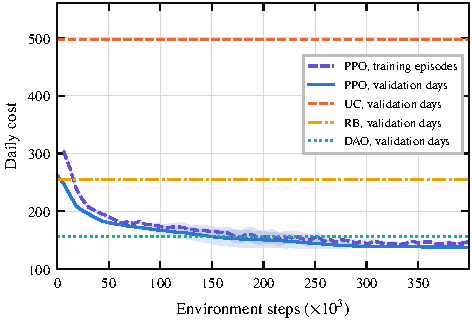
\includegraphics[width=\columnwidth]{fig_learning.pdf}
\caption{PPO learning curves (mean and $\pm1$ standard deviation over
\NSeed{} seeds) on training episodes and on ten fixed validation days,
with the benchmark costs on the validation days.}
\label{fig:learning}
\end{figure}

\subsection{Performance on Held-Out Test Days}
\label{sec:testres}

Table~\ref{tab:test} summarizes the 30 test days. PPO attains a mean
daily cost of \TPPOCost, which is \TRedCostDAO\% lower than DAO,
\TRedCostRB\% lower than RB, and \TRedCostUC\% lower than UC. The
seed-averaged PPO cost is lower than that of DAO on \TWinsDAO{} of the
30 days and lower than that of RB and UC on \TWinsRB{} and \TWinsUC{}
days, respectively, and the paired Wilcoxon signed-rank test on the seed-averaged
daily costs gives $p=\TPDAO$ against each benchmark.

\begin{table*}[!t]
\caption{Results on the 30 held-out test days (mean $\pm$ standard deviation across days). PPO values are pooled over 5 seeds; the value in parentheses is the standard deviation of the per-seed means.}
\label{tab:test}
\centering
\footnotesize
\begin{tabular}{lcccc}
\toprule
\textbf{Metric} & \textbf{UC} & \textbf{RB} & \textbf{DAO} & \textbf{PPO (proposed)}\\
\midrule
Daily cost $\sum_t c_t$ & 477.2 $\pm$ 74.8 & 245.5 $\pm$ 31.6 & 152.3 $\pm$ 31.8 & 135.5 $\pm$ 26.0 (1.3) \\
Voltage-violation hours (h) & 19.3 $\pm$ 3.4 & 12.5 $\pm$ 2.1 & 18.2 $\pm$ 4.0 & 11.9 $\pm$ 5.5 (1.1) \\
Undervoltage (p.u.$\cdot$h) & 7.40 $\pm$ 1.49 & 2.86 $\pm$ 0.59 & 1.04 $\pm$ 0.37 & 0.90 $\pm$ 0.35 (0.01) \\
Overvoltage (p.u.$\cdot$h) & 0.050 $\pm$ 0.082 & 0.001 $\pm$ 0.005 & 0.001 $\pm$ 0.005 & 0.004 $\pm$ 0.016 (0.001) \\
Minimum voltage (p.u.) & 0.835 $\pm$ 0.015 & 0.907 $\pm$ 0.007 & 0.922 $\pm$ 0.007 & 0.925 $\pm$ 0.006 (0.000) \\
Maximum voltage (p.u.) & 1.044 $\pm$ 0.028 & 1.024 $\pm$ 0.016 & 1.029 $\pm$ 0.019 & 1.024 $\pm$ 0.022 (0.000) \\
Mean hourly nadir (mHz) & 54.4 $\pm$ 6.2 & 49.4 $\pm$ 6.0 & 49.8 $\pm$ 6.0 & 47.3 $\pm$ 5.9 (0.1) \\
Worst nadir (mHz) & 79.2 $\pm$ 10.4 & 70.5 $\pm$ 7.6 & 70.5 $\pm$ 7.6 & 69.6 $\pm$ 7.5 (0.4) \\
RMS frequency deviation (mHz) & 12.80 $\pm$ 1.22 & 11.48 $\pm$ 1.16 & 11.57 $\pm$ 1.18 & 10.87 $\pm$ 1.10 (0.01) \\
Maximum RoCoF (Hz/s) & 0.154 $\pm$ 0.024 & 0.137 $\pm$ 0.016 & 0.137 $\pm$ 0.016 & 0.133 $\pm$ 0.015 (0.001) \\
RMS tie-line deviation (MW) & 2.51 $\pm$ 0.23 & 2.49 $\pm$ 0.24 & 2.49 $\pm$ 0.24 & 2.51 $\pm$ 0.25 (0.00) \\
Mean V2G reserve, both areas (MW) & 0.0 $\pm$ 0.0 & 15.2 $\pm$ 1.4 & 13.9 $\pm$ 2.6 & 25.3 $\pm$ 2.8 (0.3) \\
Fleet throughput, area level (MWh) & 491 $\pm$ 19 & 337 $\pm$ 92 & 348 $\pm$ 26 & 446 $\pm$ 39 (3) \\
Terminal SoC deficit (\%) & 0.00 $\pm$ 0.00 & 13.58 $\pm$ 14.06 & 9.68 $\pm$ 13.55 & 6.31 $\pm$ 6.80 (0.69) \\
Projection events per day & 27.8 $\pm$ 5.0 & 0.0 $\pm$ 0.0 & 1.6 $\pm$ 2.8 & 0.0 $\pm$ 0.0 (0.0) \\
Energy loss, two feeders (MWh) & 4.978 $\pm$ 0.595 & 3.416 $\pm$ 0.261 & 3.217 $\pm$ 0.338 & 3.159 $\pm$ 0.357 (0.015) \\
Unmet mobility energy (MWh) & 0.00 $\pm$ 0.00 & 0.00 $\pm$ 0.00 & 1.28 $\pm$ 2.55 & 0.00 $\pm$ 0.00 (0.00) \\
\bottomrule
\end{tabular}
\end{table*}


\emph{Voltage.} Uncontrolled charging coincides with the residential
evening peak and drives the Area~1 voltage down to \TUCVminDay~p.u.\ on
average, with \TUCUvPuH~p.u.$\cdot$h of integrated undervoltage per
day. PPO reduces the undervoltage to \TPPOUvPuH~p.u.$\cdot$h, which is
\TRedUvPuHUC\% below UC, \TRedUvPuHRB\% below RB, and \TRedUvPuHDAO\%
below DAO, and it lowers the number of violation hours from
\TDAOViolHours{} with DAO to \TPPOViolHours. Most of the remaining
violation hours are shallow (a few thousandths of a per unit) on the
Area~1 feeder. Deeper violations remain in Area~2 between 18:00 and
21:00, when only a small part of the workplace fleet is still plugged
in (Fig.~\ref{fig:heatmap}). Overvoltage is rare for all
controllers on the test days because the Area~2 workplace fleet
absorbs midday PV; the PPO maximum voltage is \TPPOVmaxDay~p.u.

\emph{Frequency.} PPO holds an average of \TPPOReserveMeanMw~MW of V2G
reserve across both areas, against \TRBReserveMeanMw~MW for RB and \TDAOReserveMeanMw~MW for DAO,
which hold a fixed 30\% share. The mean hourly nadir falls from
\TUCNadirMeanHz~mHz with UC to \TPPONadirMeanHz~mHz, and it is
\TRedNadirMeanHzDAO\% lower than with DAO. The maximum RoCoF decreases
by \TRedRocofMaxUC\% relative to UC. These gains are modest in absolute
terms because the V2G reserve is a small fraction of the 500-MW area
base and the governors respond within about one second. They are
nonetheless obtained without degrading the voltage objective, which is
the point of the joint allocation.

\emph{Energy and fleet.} PPO leaves a terminal SoC deficit of
\TPPOSocDefPct\%, against \TDAOSocDefPct\% for DAO and \TRBSocDefPct\%
for RB. Its fleet throughput, \TPPOThroughputMwh~MWh at area level, is
higher than that of DAO (\TDAOThroughputMwh~MWh) and RB because the
policy charges during the day to supply the evening discharge.
Section~\ref{sec:regenergy} examines the energy and power limits in
detail.

\subsection{Regulation Energy, Treatment Sensitivity, and Feasibility Audit}
\label{sec:regenergy}

\emph{Physical interpretation of the hourly extrapolation.} The 60-s
window of each hour contains one step load change at $t=2$~s and a
continuous fluctuation. Multiplying the window energy by 60 therefore
assumes that the step event recurs every minute, whereas the model
defines one step per hour. The exact 3600-s simulations recorded for
every evaluated hour show how large the error is. For the PPO
policies the gross regulation energy over the test days is
\TrkPPOGrossFull~MWh per day in the exact simulation, against
\TrkPPOGrossHour~MWh with the hourly extrapolation
(\TrkPPOGrossHourRatio{} times too large) and \TrkPPOGrossWin~MWh with
the window alone (more than 20 times too small). The decomposed
treatment \eqref{eq:decomposed} gives \TrkPPOGrossDec~MWh, or
\TrkPPOGrossDecRatio{} of the exact value. The same ratio of
\TrkRBGrossDecRatio{} to \TrkDAOGrossDecRatio{} is found for RB and
DAO, so the remaining 6\% shortfall is systematic rather than random.
A likely cause, which we state as an interpretation, is that the
fluctuation-only window starts from rest, so that its first seconds
under-represent the stationary fluctuation before the scaling to 59
minutes. The net daily energies are
\TrkPPONetFull~MWh (exact), \TrkPPONetDec~MWh (decomposed),
\TrkPPONetHour~MWh (hourly extrapolation), and \TrkPPONetWin~MWh
(window). The hourly extrapolation also gets the sign of the hourly
net energy wrong in \TrkPPOSignFlipPct\% of the hours, because the sign
of the single step event dominates the window while the full hour is
dominated by the fluctuation and by the lossy round trips. The same
ratios are found for RB and DAO (gross ratio \TrkRBGrossHourRatio{} and
\TrkDAOGrossHourRatio{} for the extrapolation, \TrkRBGrossDecRatio{}
and \TrkDAOGrossDecRatio{} for the decomposition). Repeating the 60-s
response for an entire hour is therefore not a physically justified
treatment: it overstates both the gross and the net regulation energy
by a factor of about two to three, and it is not simply conservative,
because its error has either sign hour by hour. The decomposed
treatment is closer to the exact simulation than any other cheap
treatment but underestimates the gross energy by about 6\%.

\emph{Sensitivity of the results to the treatment.}
Table~\ref{tab:modes} evaluates every controller on the same 30 test
days under the five treatments. For PPO, the daily cost changes by at
most \ModeDeltaCostHour{} between any treatment and the default, which
is \ModeDeltaCostSdHour{} times the seed-to-seed standard deviation of
the final policies (\PPOSeedSd); the undervoltage and the violation hours change by at
most 0.001~p.u.$\cdot$h and 0.1~h, the nadir is unchanged to the
reported precision, and the terminal SoC deficit moves between
\ModeNonePPOSocDefPct\% (neglected) and \ModeHourPPOSocDefPct\%
(hourly extrapolation). No treatment produces an SoC-limit violation
or any additional unmet mobility energy for any controller; the unmet
energy of DAO (\ModeDecomposedDAOUnmetMwh~MWh) is caused by its
schedule and is the same under all treatments to within 0.03~MWh. The regulation-energy assumption therefore does not change
the control problem, the ranking of the controllers, or any
conclusion of this paper. The decomposed treatment is retained as the
default because it tracks the exact simulation to within 6\% at the
cost of one additional 60-s simulation per hour.

\begin{table*}[!t]
\caption{Sensitivity of the daily results on the 30 test days to the treatment of the regulation energy. Every row uses the same scenarios, disturbances and controllers; only the energy credited to the droop loop in \eqref{eq:energy} differs. PPO rows pool the five final policies. The last column is the energy by which the stored energy would have left $[E^{\min},E^{\max}]$ without the limit.}
\label{tab:modes}
\centering
\scriptsize
\setlength{\tabcolsep}{3pt}
\begin{tabular}{llcccccccc}
\toprule
\textbf{Controller} & \textbf{Treatment} & \textbf{Cost} & \textbf{SoC def. (\%)} & \textbf{Unmet (MWh)} & \textbf{UV (p.u.$\cdot$h)} & \textbf{Viol. h} & \textbf{Nadir (mHz)} & \textbf{Reg. energy (MWh/d)} & \textbf{Limit viol. (MWh)}\\
\midrule
\multirow{5}{*}{UC} & None (neglected) & 477.2 & 0.00 & 0.00 & 7.402 & 19.3 & 54.4 & 0.00 & 0.000 \\
& 60-s window only & 477.2 & 0.00 & 0.00 & 7.402 & 19.3 & 54.4 & 0.00 & 0.000 \\
& Hourly extrapolation ($\times 60$) & 477.2 & 0.00 & 0.00 & 7.402 & 19.3 & 54.4 & 0.00 & 0.000 \\
& Decomposed (default) & 477.2 & 0.00 & 0.00 & 7.402 & 19.3 & 54.4 & 0.00 & 0.000 \\
& Exact 3600-s simulation & 477.2 & 0.00 & 0.00 & 7.402 & 19.3 & 54.4 & 0.00 & 0.000 \\
\midrule
\multirow{5}{*}{RB} & None (neglected) & 245.0 & 13.71 & 0.00 & 2.848 & 12.5 & 49.4 & 0.00 & 0.000 \\
& 60-s window only & 245.0 & 13.72 & 0.00 & 2.848 & 12.5 & 49.4 & -0.02 & 0.000 \\
& Hourly extrapolation ($\times 60$) & 247.0 & 13.66 & 0.00 & 2.887 & 12.6 & 49.4 & -1.10 & 0.000 \\
& Decomposed (default) & 245.5 & 13.58 & 0.00 & 2.860 & 12.5 & 49.4 & -0.46 & 0.000 \\
& Exact 3600-s simulation & 245.1 & 13.75 & 0.00 & 2.848 & 12.5 & 49.4 & -0.50 & 0.000 \\
\midrule
\multirow{5}{*}{DAO} & None (neglected) & 152.2 & 9.59 & 1.28 & 1.045 & 18.2 & 49.8 & 0.00 & 0.000 \\
& 60-s window only & 152.2 & 9.59 & 1.28 & 1.045 & 18.2 & 49.8 & -0.02 & 0.000 \\
& Hourly extrapolation ($\times 60$) & 152.5 & 9.92 & 1.30 & 1.045 & 18.2 & 49.8 & -1.02 & 0.000 \\
& Decomposed (default) & 152.3 & 9.68 & 1.28 & 1.045 & 18.2 & 49.8 & -0.43 & 0.000 \\
& Exact 3600-s simulation & 152.3 & 9.68 & 1.28 & 1.045 & 18.2 & 49.8 & -0.47 & 0.000 \\
\midrule
\multirow{5}{*}{PPO (proposed)} & None (neglected) & 135.5 & 6.26 & 0.00 & 0.904 & 11.9 & 47.3 & 0.00 & 0.000 \\
& 60-s window only & 135.5 & 6.26 & 0.00 & 0.904 & 11.9 & 47.3 & -0.03 & 0.000 \\
& Hourly extrapolation ($\times 60$) & 135.6 & 6.42 & 0.00 & 0.905 & 12.0 & 47.3 & -1.67 & 0.000 \\
& Decomposed (default) & 135.5 & 6.31 & 0.00 & 0.904 & 11.9 & 47.3 & -0.69 & 0.000 \\
& Exact 3600-s simulation & 135.5 & 6.30 & 0.00 & 0.904 & 11.9 & 47.3 & -0.73 & 0.000 \\
\bottomrule
\end{tabular}
\end{table*}


\emph{Magnitude of the term.} Table~\ref{tab:regenergy} reports the
regulation energy of the default treatment on the test days. For PPO it
averages \RegPPOHrMean~MWh per hour in absolute value over both areas,
with a maximum of \RegPPOHrMax~MWh in one hour; the gross daily energy
is \RegPPOShareGross\% of the battery energy moved by the scheduled
set-points, and the largest net change of one area fleet over a day is
\RegPPOSocAreaMax{} percentage points of its capacity. The mean net
energy is negative for every controller that holds reserve, because
each round trip is lossy, but \RegPPOPosDaysPct\% of the PPO seed-days
end with a small net gain, depending on the signs of the load steps.

\begin{table*}[!t]
\caption{Energy exchanged by the V2G droop loop and feasibility audit on the test days (area level, both areas). Regulation energy is the battery-side energy including $\eta_{\mathrm{ch}}$ and $\eta_{\mathrm{dis}}$; negative values reduce stored energy. Values use the default decomposed treatment \eqref{eq:decomposed}; the window-only column counts the simulated 60~s. The share is the gross (absolute) regulation energy relative to the battery energy of the scheduled set-points. Counts are summed over all test days (and seeds for PPO); action-clipping counts refer to individual action components.}
\label{tab:regenergy}
\centering
\scriptsize
\setlength{\tabcolsep}{2.5pt}
\begin{tabular}{lccccccccc}
\toprule
& \multicolumn{5}{c}{\textbf{Regulation energy}} & \multicolumn{4}{c}{\textbf{Feasibility audit}}\\
\cmidrule(lr){2-6}\cmidrule(lr){7-10}
\textbf{Controller} & \textbf{Mean $|\cdot|$ per h} & \textbf{Max $|\cdot|$ per h} & \textbf{Daily sum} & \textbf{Daily sum, window} & \textbf{Gross share of} & \textbf{Raw action} & \textbf{Power} & \textbf{Max power} & \textbf{Max SoC-limit}\\
 & \textbf{(MWh)} & \textbf{(MWh)} & \textbf{(MWh)} & \textbf{only (MWh)} & \textbf{sched. (\%)} & \textbf{clippings} & \textbf{projections} & \textbf{excess (MW)} & \textbf{violation (MWh)}\\
\midrule
UC & 0.000 & 0.000 & 0.00 $\pm$ 0.00 & 0.0000 & 0.00 & 0 & 833 & 0.000 & 0.000 \\
RB & 0.059 & 0.398 & -0.46 $\pm$ 0.44 & -0.0184 & 0.43 & 0 & 0 & 0.000 & 0.000 \\
DAO & 0.056 & 0.398 & -0.43 $\pm$ 0.43 & -0.0172 & 0.40 & 0 & 48 & 0.000 & 0.000 \\
PPO (proposed) & 0.091 & 0.607 & -0.69 $\pm$ 0.68 & -0.0278 & 0.51 & 7080 & 0 & 0.000 & 0.000 \\
\bottomrule
\end{tabular}
\end{table*}


\emph{Feasibility under sustained activation.} The audit columns of
Table~\ref{tab:regenergy} and the exact simulations confirm the
guarantees of Section~\ref{sec:obsact}. Over all test and stress days
and all treatments, the scheduled power plus the instantaneous droop
power never exceeds the charger or energy limits (largest excess
\TPPOPwExcess~MW), the droop power never exceeds the committed reserve,
no SoC limit is violated, and the energy balance \eqref{eq:energy}
closes to within \RegClosureMax~MWh in every hour. The
sustained-activation margin, that is, the energy that would remain
above $E^{\min}$ (or below $E^{\max}$) if the full reserve were
activated in one direction for the whole hour, is never negative. Its
minimum is exactly zero: for PPO, \eqref{eq:rup} or \eqref{eq:rdn}
limits the reserve in \TrkPPOBindHours{} feeder-hours per day on
average, and for DAO the zero margins (\TrkDAOBindHours{} feeder-hours
per day) all occur in hours with a mobility shortfall, where no upward
reserve is credited by design. In the exact 3600-s simulations the droop
power reaches its saturation limit in \TrkPPOSatFrac\% of the simulated
time, so the actual activation stays far below the sustained worst
case that the design limit protects against. Projection events occur
for UC (\TUCProj{} on the test days), which requests full charging
until the fleet is full, and occasionally for DAO (\TDAOProj), whose
open-loop schedule does not see the realized regulation energy; they do
not occur for RB or PPO.

\subsection{Raw-Action Saturation and a Bounded-Action Policy}
\label{sec:clip}

Table~\ref{tab:clip} reports, for each action dimension, how often the
deterministic action of the final policies lies outside $[-1,1]$
before clipping. Over the \ClipDimSteps{} hourly decisions of the five
policies on the test days, \ClipDimAll\% of the action components are
saturated: \ClipDimPsetOne\% for the Area~1 set-point (\ClipAbovePsetOne\%
above, \ClipBelowPsetOne\% below), \ClipDimPsetTwo\% for the Area~2
set-point, \ClipDimRhoOne\% for the Area~1 reserve share (mostly above,
that is, at $\rho_{\max}$) and \ClipDimRhoTwo\% for the Area~2 share.
The median excess beyond the bound is \ClipMedianExcess. These
saturations correspond to charging or discharging at the full available
rating, or to the minimum or maximum reserve share, which are admissible
operating points because the action bounds coincide with the design
limits; none of them is a physically infeasible request, as the zero
projection count for PPO shows. The high rate does, however, mean that
the Gaussian mean often lies well outside the box, so the gradient of
the clipped action with respect to the policy parameters is zero in
those states and exploration there is wasted.

To test whether a properly bounded policy performs better, a policy
with a hyperbolic-tangent squashed output and generalized
state-dependent exploration \cite{Raffin2022} was trained with three
seeds and the same 200\,000-step budget as the ablation reference, with
all other hyperparameters unchanged. Its action is bounded by
construction (saturation \ClipSquashAll\%). Its test cost is
\AblSquashCost~$\pm$~\AblSquashCostSd{} against \AblRefCost~$\pm$~\AblRefCostSd{}
for the clipped Gaussian reference (seed costs \AblSquashSeedCosts{}
versus \AblRefSeedCosts), with higher undervoltage
(\AblSquashUvPuH~p.u.$\cdot$h against \AblRefUvPuH) and a larger
terminal SoC deficit (\AblSquashSocDefPct\% against \AblRefSocDefPct\%).
Its learning curves plateau early, at a validation cost near the
final value from about 50\,000 steps, and change by at most
\AblSquashConvMax\% over the last 50\,000 steps, whereas the clipped
reference is still improving at the same point. Our interpretation,
which we have not tested further, is that the squashing compresses
the policy gradient near the bounds, which are precisely the
operating points that the task rewards, so that the bounded policy
settles in a worse region of the decision space. We therefore keep
the clipped Gaussian policy for the main results, report its saturation
statistics openly, and note that a longer training budget, different
exploration settings, or a Beta-distributed policy could change this
comparison.

\begin{table*}[!t]
\caption{Raw-action saturation per action dimension on the test days (percentage of hourly decisions whose deterministic action lies outside $[-1,1]$ before clipping; for the squashed policy the action is bounded by construction) and the resulting performance. Seeds in parentheses.}
\label{tab:clip}
\centering
\scriptsize
\setlength{\tabcolsep}{3pt}
\begin{tabular}{lcccccccccc}
\toprule
\textbf{Policy (seeds)} & $a_1$ ($P_1$) & $a_2$ ($P_2$) & $a_3$ ($\rho_1$) & $a_4$ ($\rho_2$) & \textbf{All} & \textbf{Cost} & \textbf{UV (p.u.$\cdot$h)} & \textbf{Nadir (mHz)} & \textbf{Reserve (MW)} & \textbf{SoC def. (\%)}\\
\midrule
Clipped Gaussian (reference, 200k) (3) & 38.3 & 50.5 & 41.5 & 37.6 & 42.0 & 147.3 $\pm$ 10.7 & 0.92 & 47.8 & 22.9 & 15.62 \\
Squashed Gaussian + gSDE (200k) (3) & 0.0 & 0.0 & 0.0 & 0.0 & 0.0 & 178.4 $\pm$ 0.4 & 1.18 & 48.9 & 18.6 & 28.14 \\
Clipped Gaussian (final, 400k) (5) & 38.5 & 55.5 & 54.0 & 48.6 & 49.2 & 135.5 $\pm$ 1.3 & 0.90 & 47.3 & 25.3 & 6.31 \\
\bottomrule
\end{tabular}
\end{table*}


\subsection{Operating Behavior on a Representative Day}
\label{sec:day}

Fig.~\ref{fig:day} shows the first test day. Under UC, the Area~1
minimum voltage falls to \DayUCVminOne~p.u.\ at 19:00 because arriving
vehicles charge at full rate during the peak. RB discharges once the
forecast voltage crosses its threshold, but its night-time charging at
full rate pulls the voltage below \DayRBNightVmin~p.u.\ between midnight and
05:00. DAO keeps the voltage close to the 0.95~p.u.\ limit throughout,
as its foresight allows. PPO begins discharging in Area~1 at about 17:00,
when the minimum voltage reaches the 0.95~p.u.\ limit, reaches about
\DayPPOPeakOne~MW at 19:00, and
recharges at a moderate rate overnight, so the minimum voltage stays
near 0.95~p.u.\ and the Area~1 SoC ends the day close to its initial
value. In Area~2, PPO charges while the workplace fleet is plugged in
(06:00 to 15:00, largely from PV), starts discharging at 16:00, and
discharges at the full plugged-in rating at 17:00, just before the
fleet leaves.
Fig.~\ref{fig:day}(f) shows that PPO keeps \DayResLo{} to \DayResHi~MW of reserve for
most of the day and reduces it at 17:00 to 19:00, when the converter
capacity is needed for discharge. The voltage maps in
Fig.~\ref{fig:heatmap} show that the deep undervoltage on the main
feeder and the bus 26 to 33 lateral of Area~1 is removed, while the
evening undervoltage in Area~2 is reduced but not eliminated.

\begin{figure*}[!t]
\centering
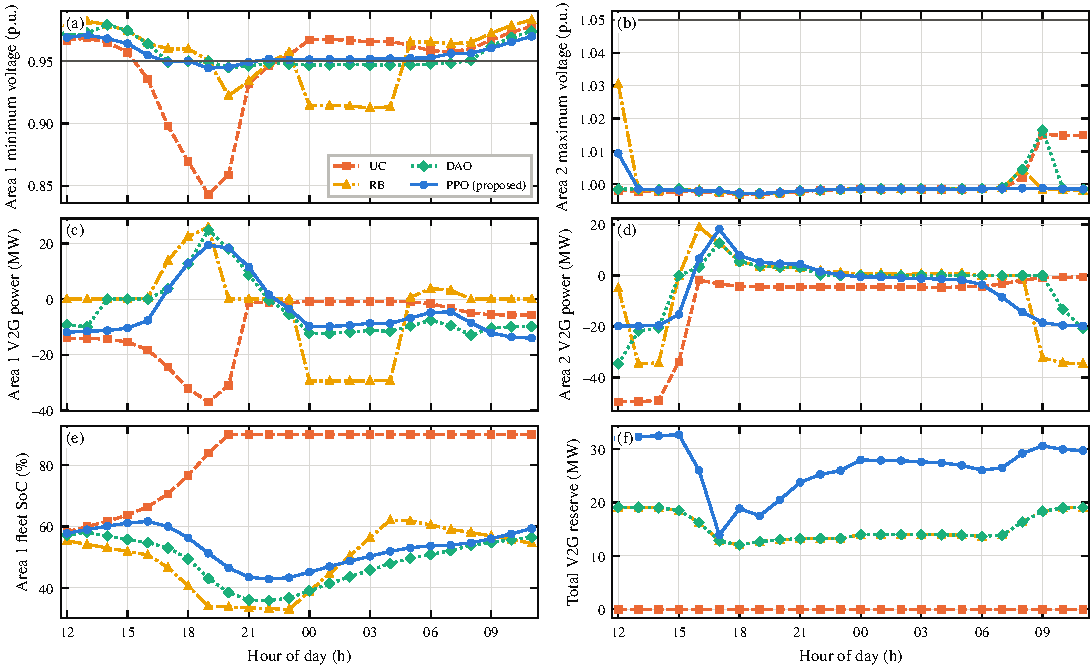
\includegraphics[width=\textwidth]{fig_day.pdf}
\caption{Representative test day (day 1, PPO seed 0). (a) Area~1
minimum bus voltage. (b) Area~2 maximum bus voltage. (c), (d) Area-level
V2G set-points (positive values denote discharge). (e) Area~1 fleet SoC.
(f) Total V2G frequency reserve.}
\label{fig:day}
\end{figure*}

\begin{figure*}[!t]
\centering
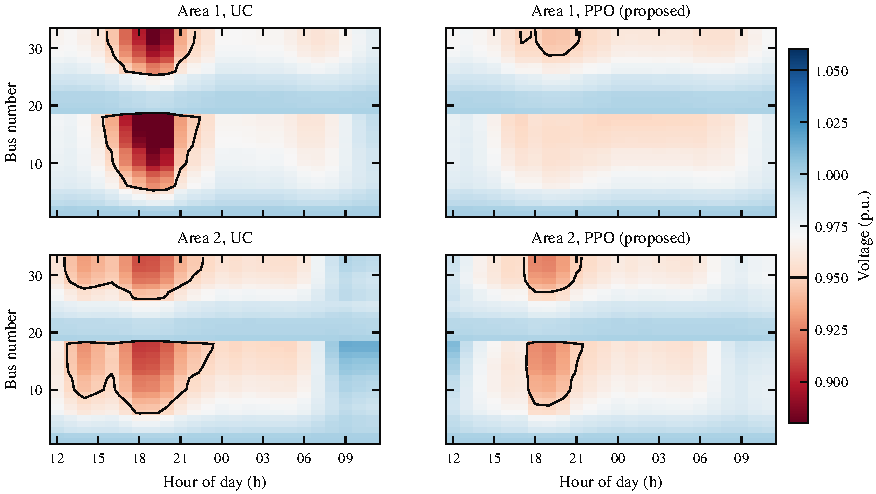
\includegraphics[width=0.9\textwidth]{fig_heatmap.pdf}
\caption{Bus voltages over the representative test day under UC and
PPO. Black contours mark 0.95 and 1.05~p.u.}
\label{fig:heatmap}
\end{figure*}

\subsection{Frequency Response Within an Hour}
\label{sec:freqres}

Fig.~\ref{fig:freq} shows the 60-s window at \FreqHour{} of the same
day. PV has reduced the inertia constant of Area~2 to \HrHtwo~s, and a
load step occurs in Area~1 at $t=2$~s; Area~2 sees the disturbance
through the tie line. Without reserve (UC), the Area~2 nadir
reaches \HrUCNadirTwo~mHz and the inter-area oscillation is lightly
damped. PPO holds \HrPPORes~MW of reserve at this hour, most of it in
Area~2 where the workplace fleet is connected, against \HrRBRes~MW for
RB. The Area~2 nadir is reduced to \HrPPONadirTwo~mHz (\HrRBNadirTwo~mHz with RB) and the oscillation
decays faster. The Area~1 nadir changes much less (\HrUCNadirOne, \HrRBNadirOne, and \HrPPONadirOne~mHz for UC,
RB, and PPO), because only about a quarter of the residential fleet is
plugged in at midday and PPO assigns it a small reserve share. The worst nadir over
the two areas in this hour is therefore \HrPPONadir~mHz for PPO and
\HrRBNadir~mHz for RB. This example shows that the benefit of reserve
depends on where the disturbance occurs relative to where the reserve
is held, which is why the test-set gains in Table~\ref{tab:test} are
averages over random disturbance locations.

\begin{figure*}[!t]
\centering
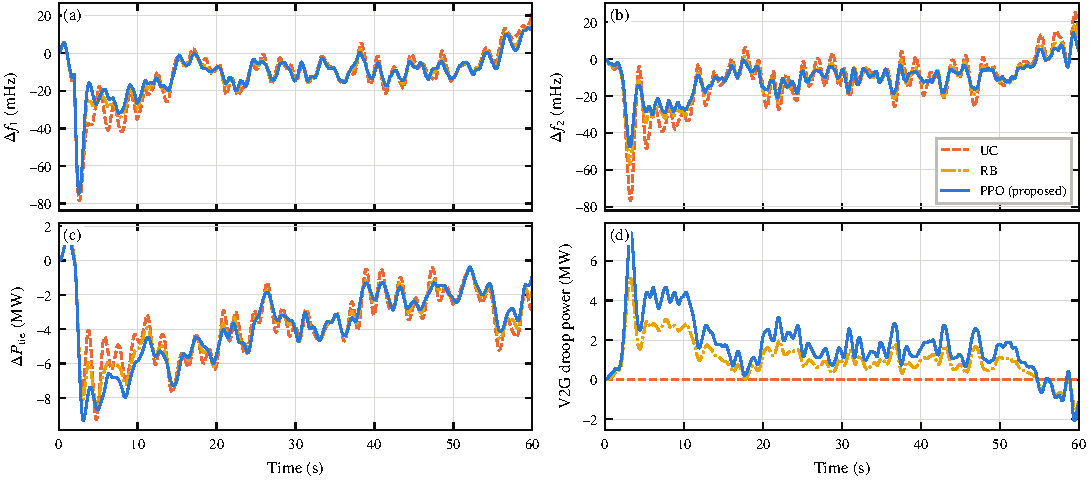
\includegraphics[width=\textwidth]{fig_freq.pdf}
\caption{Frequency response at \FreqHour{} of the representative day.
(a), (b) Area frequency deviations. (c) Tie-line power deviation.
(d) Total V2G droop power.}
\label{fig:freq}
\end{figure*}

\subsection{Learned Allocation Between Voltage Support and Reserve}
\label{sec:alloc}

Fig.~\ref{fig:policy} averages the PPO decisions over all test days and
seeds. The reserve share follows fleet availability more than inertia. In
Area~2, the policy holds $\rho\approx\RhoMidTwo$ between 10:00 and
14:00, when the workplace fleet is connected and PV has lowered the
inertia, and releases the reserve to zero in the evening, when the
few remaining vehicles are discharged to support the feeder voltage.
In Area~1, the reserve share is close to its upper limit at night
($\rho\approx\RhoNightOne$), when inertia is high but the residential
fleet is plugged in and otherwise idle, drops to \RhoMidOne{} at midday, when most
residential vehicles are away and the remaining ones charge, and settles
near \RhoEveOne{} during the evening peak, when part of the converter
capacity is used for discharge. The set-points show charging from
midday PV in both areas, discharge in the evening peak, and moderate
overnight charging in Area~1. None of these rules was specified in the
reward; they emerge from the trade-off encoded in \eqref{eq:cost}.

\begin{figure}[!t]
\centering
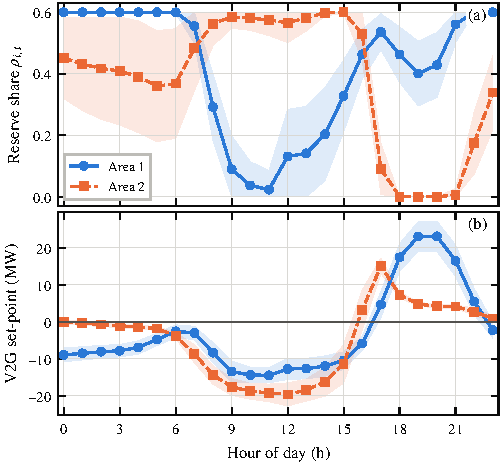
\includegraphics[width=\columnwidth]{fig_policy.pdf}
\caption{PPO decisions averaged over the test days and \NSeed{} seeds
(mean and $\pm1$ standard deviation). (a) Reserve share. (b) Area-level
V2G set-point.}
\label{fig:policy}
\end{figure}

\begin{figure*}[!t]
\centering
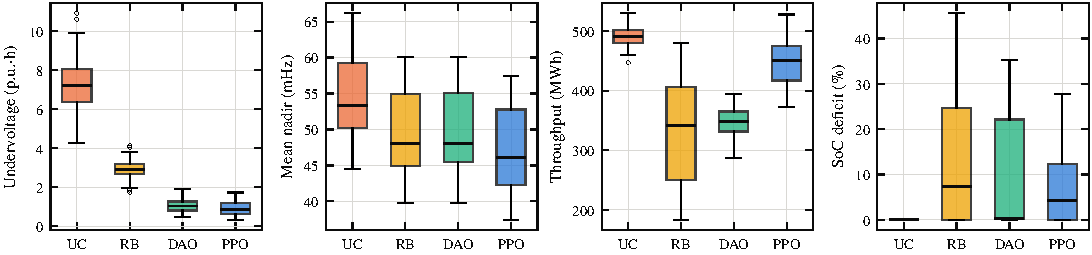
\includegraphics[width=\textwidth]{fig_box.pdf}
\caption{Distribution of daily metrics over the test days (PPO pooled
over \NSeed{} seeds).}
\label{fig:box}
\end{figure*}

Fig.~\ref{fig:box} shows the distributions behind the averages. The
undervoltage distribution of PPO lies below those of RB and DAO, and
its throughput is higher. Its mean SoC deficit is lower than that of RB
and DAO, but the median is not: DAO ends \TDAOSocDefZeroPct\% of the days with no
deficit (median \TDAOSocDefMedian\%), whereas PPO tends to leave a small deficit on many days (median \TPPOSocDefMedian\%). The nadir distributions of
all controllers overlap, because the day-to-day variation of the
disturbance size is larger than the effect of the reserve; compared
day by day, however, the PPO mean nadir is lower than that of DAO on
\TNadirWinsDAO{} of the 30 test days, than that of RB on \TNadirWinsRB,
and than that of UC on \TNadirWinsUC{} (paired Wilcoxon test against
DAO, $p=\TNadirPDAO$).

\subsection{Out-of-Distribution Stress Days}
\label{sec:stress}

Table~\ref{tab:stress} reports the 20 stress days, which combine 10\% to
20\% heavier load, 30\% to 45\% lower fleet participation, and larger
disturbances, all beyond the training ranges, with clear-sky PV. All controllers deteriorate. PPO remains the
lowest-cost controller, \SRedCostDAO\% below DAO and \SRedCostRB\% below
RB, and its daily cost is the lowest on all 20 days ($p=\SPDAO$ against
each benchmark). Its undervoltage is \SRedUvPuHDAO\% below DAO. The
policy does, however, show several signs of operating outside its
training range. It records more violation hours than RB
(\SPPOViolHours{} against \SRBViolHours), because it spreads the
limited fleet energy over more hours with shallow violations, its
terminal SoC deficit rises to \SPPOSocDefPct\%, and its maximum voltage
reaches \SPPOVmaxDay~p.u. Training on a wider scenario distribution, or
adding a hard terminal-energy constraint, would be needed before
deployment under such conditions.

\begin{table*}[!t]
\caption{Results on the 20 out-of-distribution stress days (mean $\pm$ standard deviation across days). PPO values are pooled over 5 seeds; the value in parentheses is the standard deviation of the per-seed means.}
\label{tab:stress}
\centering
\footnotesize
\begin{tabular}{lcccc}
\toprule
\textbf{Metric} & \textbf{UC} & \textbf{RB} & \textbf{DAO} & \textbf{PPO (proposed)}\\
\midrule
Daily cost $\sum_t c_t$ & 671.4 $\pm$ 24.3 & 369.4 $\pm$ 17.6 & 308.3 $\pm$ 19.6 & 283.8 $\pm$ 16.2 (3.1) \\
Voltage-violation hours (h) & 24.3 $\pm$ 2.3 & 14.2 $\pm$ 1.3 & 18.6 $\pm$ 4.5 & 18.5 $\pm$ 3.0 (1.0) \\
Undervoltage (p.u.$\cdot$h) & 10.25 $\pm$ 0.50 & 4.15 $\pm$ 0.36 & 2.88 $\pm$ 0.29 & 2.66 $\pm$ 0.27 (0.13) \\
Overvoltage (p.u.$\cdot$h) & 0.070 $\pm$ 0.024 & 0.000 $\pm$ 0.001 & 0.000 $\pm$ 0.001 & 0.006 $\pm$ 0.009 (0.003) \\
Minimum voltage (p.u.) & 0.835 $\pm$ 0.006 & 0.898 $\pm$ 0.003 & 0.903 $\pm$ 0.004 & 0.905 $\pm$ 0.004 (0.000) \\
Maximum voltage (p.u.) & 1.070 $\pm$ 0.004 & 1.043 $\pm$ 0.005 & 1.048 $\pm$ 0.002 & 1.052 $\pm$ 0.005 (0.002) \\
Mean hourly nadir (mHz) & 82.6 $\pm$ 6.4 & 76.8 $\pm$ 6.2 & 77.6 $\pm$ 6.3 & 75.0 $\pm$ 6.1 (0.4) \\
Worst nadir (mHz) & 121.3 $\pm$ 11.5 & 108.6 $\pm$ 9.9 & 108.6 $\pm$ 10.0 & 105.8 $\pm$ 9.3 (0.5) \\
Maximum RoCoF (Hz/s) & 0.240 $\pm$ 0.021 & 0.215 $\pm$ 0.018 & 0.215 $\pm$ 0.018 & 0.205 $\pm$ 0.019 (0.002) \\
Terminal SoC deficit (\%) & 0.00 $\pm$ 0.00 & 26.16 $\pm$ 3.65 & 24.30 $\pm$ 8.70 & 18.02 $\pm$ 4.07 (2.94) \\
Projection events per day & 16.4 $\pm$ 1.0 & 0.0 $\pm$ 0.0 & 2.8 $\pm$ 3.0 & 0.0 $\pm$ 0.0 (0.0) \\
Unmet mobility energy (MWh) & 0.00 $\pm$ 0.00 & 0.00 $\pm$ 0.00 & 2.43 $\pm$ 2.76 & 0.00 $\pm$ 0.00 (0.00) \\
\bottomrule
\end{tabular}
\end{table*}


\subsection{Reward Ablation and Weight Sensitivity}
\label{sec:ablation}

Tables~\ref{tab:ablation} and \ref{tab:sensitivity} report policies
trained with one reward term removed, or with the voltage or frequency
weight halved and doubled, and evaluated with the nominal cost
\eqref{eq:cost}. To limit computation each variant was trained for
200\,000 steps, with three seeds for the ablation and two for the
sensitivity study, and a reference policy with the nominal reward was
trained under the same budget in the same environment.
The comparison is made against this reference, not against the
400\,000-step policies of Table~\ref{tab:test}. The same seed means
the same initial network weights and the same scenario stream, so the
seed-paired difference between a variant and the reference isolates the
effect of the reward change.

\emph{Frequency terms.} Removing them has a clear and consistent
effect. All three seeds give up most of the reserve
(\AblNoFReserveMeanMw~MW instead of \AblRefReserveMeanMw~MW), raise the
mean nadir from \AblRefNadirMeanHz{} to \AblNoFNadirMeanHz~mHz, and
increase the nominal cost in every seed pair (differences
\AblNoFPairDiffs; mean \AblNoFPairMean). Halving $w_f$ moves the policy
in the same direction (reserve \AblWfLowReserveMeanMw~MW, paired cost
differences \AblWfLowPairDiffs), and doubling it raises the reserve to
\AblWfHighReserveMeanMw~MW at the price of more undervoltage
(\AblWfHighUvPuH~p.u.$\cdot$h against \AblRefUvPuH). The reserve
allocation of Fig.~\ref{fig:policy} is therefore controlled by the
frequency weight, and the nominal $w_f=4$ sits between the two extremes.

\emph{Voltage weight.} Doubling $w_V$ reduces undervoltage to
\AblWvHighUvPuH~p.u.$\cdot$h but cuts the reserve by
\AblWvHighReserveRedPct\% (\AblWvHighReserveMeanMw~MW) and raises the terminal SoC deficit to
\AblWvHighSocDefPct\%, because the policy discharges more in the evening
and recharges less. Halving $w_V$ does the opposite. The two weights
thus trade voltage support against reserve and end-of-day energy in the
expected directions.

\emph{Why some variants show a lower total cost than the reference.}
Removing the overvoltage or throughput term, halving $w_V$, or
doubling $w_f$ yields a lower mean nominal cost than the reference
(Tables~\ref{tab:ablation} and \ref{tab:sensitivity}),
which at first sight suggests that these terms are harmful. The cost
decomposition shows otherwise. The voltage, frequency, and throughput
components of the reference and of these variants differ by only a few
units (voltage \AblRefCostV{} against \AblNoOVCostV{} and
\AblNoDegCostV; frequency \AblRefCostF{} against \AblNoOVCostF{} and
\AblNoDegCostF). Almost the entire difference comes from the terminal
SoC term, which is \AblRefCostTerm{} for the reference,
\AblNoOVCostTerm{} without the overvoltage term, \AblNoDegCostTerm{}
without the throughput term, \AblWvLowCostTerm{} with $w_V=25$, and
\AblWfHighCostTerm{} with $w_f=8$. This
term is paid once per episode and is the slowest part of the reward to
learn: at 200\,000 steps the three reference seeds leave terminal
deficits of \AblRefSeedSocDefs{} percentage points (seed costs
\AblRefSeedCosts), whereas the 400\,000-step policies of
Table~\ref{tab:test} reach \TPPOSocDefPct\%. The apparent advantage of the variants is therefore a
training-budget effect on a term unrelated to the removed one, and it is
not statistically distinguishable from the reference (Welch tests on
seed means, $p=\AblNoOVPval$ and $p=\AblNoDegPval$; paired differences
\AblNoOVPairDiffs{} and \AblNoDegPairDiffs). Consistent with this, the
200\,000-step runs with large terminal deficits have not met the
convergence criterion of Section~\ref{sec:ppo} (validation cost still
changing by up to \AblNoOVConvMax\% over the final 50\,000 steps). The
overvoltage term has little effect on the test days because
overvoltage is rare for every policy, and the throughput term with
$w_{\mathrm{deg}}=0.05$ is a minor part of the cost. We keep both terms
because they encode constraints that matter on days the test set does
not represent, but the evidence here does not show that they improve
performance.

\begin{table*}[!t]
\caption{Reward ablation on the test days (mean $\pm$ standard deviation across seeds). Every policy is trained for 200\,000 steps in the corrected environment with the modified reward and evaluated with the full cost \eqref{eq:cost}.}
\label{tab:ablation}
\centering
\footnotesize
\setlength{\tabcolsep}{4pt}
\begin{tabular}{lccccccc}
\toprule
\textbf{Reward variant (seeds)} & \textbf{Cost} & \textbf{UV (p.u.$\cdot$h)} & \textbf{OV (p.u.$\cdot$h)} & \textbf{Nadir (mHz)} & \textbf{Reserve (MW)} & \textbf{Thr. (MWh)} & \textbf{SoC def. (\%)}\\
\midrule
Full reward (reference) (3) & 147.3 $\pm$ 10.7 & 0.92 $\pm$ 0.03 & 0.003 $\pm$ 0.002 & 47.8 $\pm$ 0.4 & 22.9 $\pm$ 2.6 & 437 $\pm$ 25 & 15.62 $\pm$ 10.68 \\
$w_{\mathrm{ov}}=0$ (no overvoltage term) (3) & 144.4 $\pm$ 5.4 & 0.92 $\pm$ 0.02 & 0.004 $\pm$ 0.001 & 47.5 $\pm$ 0.2 & 24.4 $\pm$ 0.5 & 431 $\pm$ 32 & 13.75 $\pm$ 7.06 \\
$w_f=w_{\mathrm{tie}}=0$ (no frequency terms) (3) & 169.0 $\pm$ 0.9 & 0.86 $\pm$ 0.01 & 0.001 $\pm$ 0.000 & 51.0 $\pm$ 0.4 & 10.1 $\pm$ 1.3 & 512 $\pm$ 29 & 28.68 $\pm$ 0.36 \\
$w_{\mathrm{deg}}=0$ (no throughput term) (3) & 145.6 $\pm$ 10.3 & 0.92 $\pm$ 0.03 & 0.002 $\pm$ 0.001 & 47.8 $\pm$ 0.3 & 23.1 $\pm$ 1.9 & 452 $\pm$ 23 & 13.88 $\pm$ 10.75 \\
\bottomrule
\end{tabular}
\end{table*}

\begin{table*}[!t]
\caption{Reward-weight sensitivity on the test days (mean $\pm$ standard deviation across seeds; 200\,000 steps; evaluation with the nominal weights of Table~\ref{tab:params}).}
\label{tab:sensitivity}
\centering
\footnotesize
\setlength{\tabcolsep}{4pt}
\begin{tabular}{lccccccc}
\toprule
\textbf{Reward variant (seeds)} & \textbf{Cost} & \textbf{UV (p.u.$\cdot$h)} & \textbf{OV (p.u.$\cdot$h)} & \textbf{Nadir (mHz)} & \textbf{Reserve (MW)} & \textbf{Thr. (MWh)} & \textbf{SoC def. (\%)}\\
\midrule
Full reward (reference) (3) & 147.3 $\pm$ 10.7 & 0.92 $\pm$ 0.03 & 0.003 $\pm$ 0.002 & 47.8 $\pm$ 0.4 & 22.9 $\pm$ 2.6 & 437 $\pm$ 25 & 15.62 $\pm$ 10.68 \\
$w_V=25$ (half) (2) & 140.1 $\pm$ 0.4 & 1.09 $\pm$ 0.03 & 0.008 $\pm$ 0.003 & 47.0 $\pm$ 0.1 & 26.4 $\pm$ 0.4 & 428 $\pm$ 3 & 2.17 $\pm$ 0.78 \\
$w_V=100$ (double) (2) & 167.5 $\pm$ 0.4 & 0.85 $\pm$ 0.01 & 0.003 $\pm$ 0.002 & 49.9 $\pm$ 0.1 & 13.9 $\pm$ 0.3 & 442 $\pm$ 19 & 30.85 $\pm$ 0.28 \\
$w_f=2$ (half) (2) & 161.9 $\pm$ 5.8 & 0.87 $\pm$ 0.00 & 0.001 $\pm$ 0.001 & 49.3 $\pm$ 0.8 & 16.5 $\pm$ 3.4 & 458 $\pm$ 30 & 27.38 $\pm$ 2.56 \\
$w_f=8$ (double) (2) & 140.5 $\pm$ 0.4 & 1.00 $\pm$ 0.01 & 0.007 $\pm$ 0.001 & 46.9 $\pm$ 0.4 & 26.6 $\pm$ 1.3 & 415 $\pm$ 21 & 7.84 $\pm$ 0.90 \\
\bottomrule
\end{tabular}
\end{table*}


\subsection{Limitations}
\label{sec:limits}

Several simplifications bound the conclusions. Each area's
distribution system is represented by identical copies of one feeder,
so feeder diversity and the coupling between distribution voltages and
transmission-level frequency are not captured. The fleet is modeled as
one aggregated battery per feeder; individual departure constraints,
charger heterogeneity, and battery aging physics are not modeled, and
the throughput term is only a proxy for degradation. Reactive-power
capability of the chargers, which is effective for voltage control
\cite{HuEtAl2022}, is not used. The load, PV, and availability profiles
are synthetic, and the LFC model is linearized with representative
parameters rather than identified from a specific system. Finally, the
agent receives hour-ahead forecasts without error; forecast
uncertainty and communication delays at the aggregator level are left
for future work.

% ============================================================
\section{Conclusion}
\label{sec:conclusions}
% ============================================================

This paper formulated the coordination of V2G voltage support and
frequency reserve as a two-time-scale control problem and solved it
with PPO. The hourly decision of each area aggregator consists of a
fleet set-point and a reserve share. The set-point is evaluated by AC
power flow on IEEE 33-bus feeders and an energy-consistent fleet model,
and the reserve determines the gain and saturation of a V2G droop loop
in a dynamic two-area LFC model with inertia, governors, a tie line,
and AGC. All quantities are expressed in physical units, and the
models were verified against pandapower and closed-form results.

Across \NSeed{} training seeds and 30 held-out days, the learned policy
reduced the daily cost by \TRedCostDAO\% relative to a perfect-foresight
day-ahead optimization with fixed reserve, by \TRedCostRB\% relative to
a rule-based volt-watt and droop controller, and by \TRedCostUC\%
relative to uncontrolled charging. Undervoltage fell by
\TRedUvPuHDAO\% relative to the day-ahead optimization, the mean
frequency nadir by \TRedNadirMeanHzDAO\%, and the terminal SoC deficit
from \TDAOSocDefPct\% to \TPPOSocDefPct\%. The policy learned to hold
reserve mainly where and when vehicles are plugged in, including the
low-inertia midday hours in the workplace area, and to release it when
converter capacity is needed for voltage support. On
out-of-distribution stress days the policy kept the lowest cost but
showed larger SoC deficits and more frequent shallow violations,
which marks the limits of the training distribution.

Future work will add charger reactive power, forecast uncertainty,
heterogeneous feeders, electricity-cost terms in the objective, and
constrained RL formulations that enforce terminal energy requirements
as hard constraints.

\section*{Data and Code Availability}
The simulation environment, training and evaluation scripts, trained
policies, and the data behind every table and figure are available at
\url{https://github.com/kenoto99/v2g-ppo-two-area} (release v3.0.1;
archived on Zenodo, DOI: \url{https://doi.org/10.5281/zenodo.23851585}).

\section*{Acknowledgment}
The authors used an AI assistant (Claude, Anthropic) to help implement
and debug the simulation code and to edit the language of the
manuscript. All models, parameters, results, and interpretations were
checked by the authors, who take full responsibility for the content.
